% ============================================================================
% Draft of the "Method" and "Experiments" sections of an extension of
%   Musoni, Marin, Melzi, Castellani - A Functional Skeleton Transfer (2021).
%
% Only changes whose effect has been verified in the code are reported here.
% Every number comes from the code commit given in the comment next to it
% (repository PietroMsn/Functional-skeleton-transfer); see README.md for the
% changelog and for how to reproduce each experiment.
% ============================================================================
\documentclass[11pt]{article}

\usepackage[utf8]{inputenc}
\usepackage[T1]{fontenc}
\usepackage[margin=2.5cm]{geometry}
\usepackage{amsmath,amssymb,bm}
\usepackage{booktabs}
\usepackage{graphicx}
\usepackage{xcolor}
\usepackage[numbers]{natbib}
\usepackage{hyperref}

\newcommand{\M}{\mathcal{M}}
\newcommand{\N}{\mathcal{N}}
\newcommand{\R}{\mathbb{R}}
\newcommand{\Rspat}{\mathbf{R}}
\newcommand{\Rhat}{\widehat{\mathbf{R}}}
\newcommand{\X}{\mathbf{X}}
\newcommand{\J}{\mathbf{J}}
\newcommand{\C}{\mathbf{C}}
\newcommand{\F}{\mathbf{F}}
\newcommand{\one}{\mathbf{1}}
\newcommand{\todo}[1]{\textcolor{red}{[TODO: #1]}}

\title{A Functional Skeleton Transfer: exact solvers, skeleton priors and robustness to clothing\\[0.3em]
\large Draft -- Method and Experiments}
\author{Pietro Musoni \and Riccardo Marin \and Simone Melzi \and Umberto Castellani}
\date{\today}

\begin{document}
\maketitle

% ============================================================================
\section{Method}
\label{sec:method}
% ============================================================================

We build on the functional skeleton transfer of \citet{musoni2021functional}.
A rigged source shape $\M$ with $n_\M$ vertices $\X_\M \in \R^{n_\M \times 3}$,
skinning weights and a skeleton of $Q$ joints $\J_\M \in \R^{Q \times 3}$ with
parent map $p(\cdot)$ is given, together with an unrigged target $\N$ (a mesh or
a point cloud with vertices $\X_\N$) and a small set of corresponding landmarks.
We denote by $\Phi \in \R^{n_\M \times k_\M}$ and $\Psi \in \R^{n_\N \times k_\N}$
the first Laplace--Beltrami eigenfunctions of the two shapes, orthonormal with
respect to the lumped mass matrices $\mathbf{M}_\M$, $\mathbf{M}_\N$, so that
$\Phi^\dagger = \Phi^\top \mathbf{M}_\M$. The original pipeline
(i) fits a spatial joint regressor $\Rspat \in \R^{Q \times n_\M}$ on the
source, $\J_\M \approx \Rspat \X_\M$; (ii) estimates a functional map
$\C \in \R^{k_\M \times k_\N}$ from the target to the source with the
descriptor-preservation energy of \citet{nogneng2017informative}, refined with
spectral ICP and ZoomOut~\citep{melzi2019zoomout}; (iii) converts the regressor
to its functional form $\Rhat = \Rspat \Phi$ and transfers the skeleton as
\begin{equation}
  \J_\N = \Rhat \, \C \, \Psi^\dagger \X_\N .
  \label{eq:transfer}
\end{equation}
In this work we revisit steps (i) and (ii), which were solved with 1000
iterations of a first-order optimizer, and we add components that make the
transfer more robust to non-isometric targets, in particular clothed humans.

% ----------------------------------------------------------------------------
\subsection{Exact spatial regressor}
\label{sec:regressor}
% ----------------------------------------------------------------------------

The regressor of \citet{musoni2021functional} minimizes
\begin{equation}
  E(\Rspat) = \omega_{rec} \|\Rspat\X_\M - \J_\M\|^2
            + \omega_{loc} \|\Rspat \odot \F - \Rspat\|^2
            + \omega_{spa} \| |\F - \one| \odot \Rspat\|^2
            + \omega_{con} \|\Rspat \one_{n_\M} - \one_Q\|^2 ,
  \label{eq:regressor_energy}
\end{equation}
where $\F \in \{0,1\}^{Q \times n_\M}$ is the locality mask: $F_{qi}=1$ iff
vertex $i$ has a skinning weight above $0.1$ for both joint $q$ and its parent.

\paragraph{Redundant terms.} Since $\F$ is binary,
$\Rspat\odot\F - \Rspat = -\Rspat \odot (\one - \F) = -|\F - \one| \odot \Rspat$:
the locality and sparsity terms coincide and act as a single penalty
$\omega \|\Rspat \odot (\one - \F)\|^2$ with $\omega = \omega_{loc} + \omega_{spa}$.
We use the weights of the released implementation, $\omega_{rec} = 1$,
$\omega = 1000 + 100$, $\omega_{con} = 10$.

\paragraph{Closed-form solution.} The energy is quadratic and decouples over
the rows of $\Rspat$. For joint $q$ with row $\mathbf{r} \in \R^{n_\M}$ we stack
the data terms as $\|\mathbf{A}\mathbf{r} - \mathbf{b}\|^2$ with
\begin{equation}
  \mathbf{A} = \begin{bmatrix} \sqrt{\omega_{rec}}\, \X_\M^\top \\ \sqrt{\omega_{con}}\, \one^\top \end{bmatrix} \in \R^{4 \times n_\M},
  \qquad
  \mathbf{b} = \begin{bmatrix} \sqrt{\omega_{rec}}\, \J_{\M,q}^\top \\ \sqrt{\omega_{con}} \end{bmatrix} \in \R^{4},
\end{equation}
and split $\mathbf{r}$ into the coefficients inside ($S$) and outside ($O$) the
mask: $E_q = \|\mathbf{A}_S\mathbf{r}_S + \mathbf{A}_O\mathbf{r}_O - \mathbf{b}\|^2 + \omega \|\mathbf{r}_O\|^2$.
For fixed $\mathbf{r}_S$ the optimal $\mathbf{r}_O$ is a ridge regression which,
by the push-through identity, only requires a $4\times4$ inverse:
\begin{equation}
  \mathbf{r}_O^\star = \mathbf{A}_O^\top \left(\mathbf{A}_O\mathbf{A}_O^\top + \omega \mathbf{I}_4\right)^{-1} (\mathbf{b} - \mathbf{A}_S\mathbf{r}_S).
\end{equation}
Substituting it back gives the reduced energy
$E_q(\mathbf{r}_S) = (\mathbf{A}_S\mathbf{r}_S - \mathbf{b})^\top \mathbf{K} (\mathbf{A}_S\mathbf{r}_S - \mathbf{b})$
with $\mathbf{K} = \omega (\mathbf{A}_O\mathbf{A}_O^\top + \omega\mathbf{I}_4)^{-1} \succ 0$.
With $\mathbf{K} = \mathbf{L}\mathbf{L}^\top$, the minimizers are the solutions of
the $4 \times |S|$ least-squares problem $\mathbf{L}^\top\mathbf{A}_S \mathbf{r}_S \approx \mathbf{L}^\top \mathbf{b}$.
Since $|S| \gg 4$ the minimizer is not unique, and we select the minimum-norm
one, $\mathbf{r}_S = (\mathbf{L}^\top\mathbf{A}_S)^\dagger \mathbf{L}^\top\mathbf{b}$,
which spreads the weight over all the vertices of the mask. The whole
regressor is obtained with $Q$ small dense solves, without iterations or
hyper-parameters of an optimizer.

% ----------------------------------------------------------------------------
\subsection{Exact initial functional map}
\label{sec:fmap}
% ----------------------------------------------------------------------------

The initial $k \times k$ map ($k = 20$) minimizes
\begin{equation}
  E(\C) = \frac{\omega_d}{2} \|\C \widehat{\mathbf{D}}_\N - \widehat{\mathbf{D}}_\M\|^2
        + \omega_l \|\C \Lambda_\N - \Lambda_\M \C\|^2 ,
\end{equation}
where $\widehat{\mathbf{D}}$ are the spectral coefficients of the descriptors
(WKS~\citep{aubry2011wave} and wave kernel maps of the landmarks) and
$\Lambda$ the diagonal eigenvalue matrices. Because $\Lambda$ is diagonal,
$(\C\Lambda_\N - \Lambda_\M\C)_{ij} = C_{ij}(\lambda^\N_j - \lambda^\M_i)$ and
the energy decouples over the rows $\mathbf{c}_i$ of $\C$:
\begin{equation}
  \left(\omega_d \widehat{\mathbf{D}}_\N \widehat{\mathbf{D}}_\N^\top
        + 2\omega_l \operatorname{diag}\!\big((\bm{\lambda}^\N - \lambda^\M_i)^2\big)\right) \mathbf{c}_i
  = \omega_d \widehat{\mathbf{D}}_\N \, \widehat{\mathbf{d}}^{\M}_i ,
\end{equation}
with $\widehat{\mathbf{d}}^{\M}_i$ the $i$-th row of $\widehat{\mathbf{D}}_\M$.
This replaces the 1000 Adam iterations of the original implementation with $k$
linear systems of size $k \times k$.

% ----------------------------------------------------------------------------
\subsection{Connected spectral bases for point clouds}
\label{sec:connectivity}
% ----------------------------------------------------------------------------

For point clouds the Laplacian is built on a $k$-nearest-neighbour graph
\citep{sharp2020laplacian}. Loose garments create large gaps between surfaces
(e.g.\ between the hem of a skirt and the legs) that can split this graph into
several components. The multiplicity of the zero eigenvalue then equals the
number of components, the first eigenfunctions become indicator functions of
the components, and both the descriptors and the functional map lose their
meaning. We therefore check the connectivity of the graph and double the
number of neighbours (starting from 30, up to 240) until it is connected.

% ----------------------------------------------------------------------------
\subsection{Skeleton priors on the target}
\label{sec:priors}
% ----------------------------------------------------------------------------

The transfer of Eq.~\eqref{eq:transfer} treats every joint independently. We
optionally correct the transferred joints $\J^0$ with two priors on the bone
lengths $\ell_b(\J) = \|\J_b - \J_{p(b)}\|$, where bone $b$ is identified by its
child joint:
\begin{equation}
  E(\J, s) = \omega_{d} \|\J - \J^0\|^2
           + \omega_{sym} \!\!\sum_{(a,b) \in \mathcal{P}}\!\! \big(\ell_a(\J) - \ell_b(\J)\big)^2
           + \omega_{prop} \sum_{b} \big(\ell_b(\J) - s\, \ell_b(\J_\M)\big)^2 .
  \label{eq:priors}
\end{equation}
The \emph{symmetry} term asks mirrored bones (left and right femur, \dots) to
have the same length; the set $\mathcal{P}$ of mirrored pairs is detected
automatically on the source, by reflecting its joints with respect to the
sagittal plane through the root and pairing mutual nearest neighbours whose
parents are themselves mirrored. On SMPL this recovers the expected nine
pairs. The \emph{proportion} term asks the bone lengths to match the source
up to a global scale $s$, optimized jointly with the joints. All residuals are
lengths, so the weights are directly comparable; we use
$\omega_d = \omega_{sym} = \omega_{prop} = 1$. The problem has $3Q + 1$ unknowns
and is solved with a trust-region nonlinear least-squares method.

% ----------------------------------------------------------------------------
\subsection{Plausibility check}
\label{sec:plausibility}
% ----------------------------------------------------------------------------

The bone lengths also provide a test of the transfer that does not need any
ground truth. We compute the scale-normalized ratios
\begin{equation}
  \rho_b = \frac{\ell_b(\J_\N) / \ell_b(\J_\M)}{\sum_{b'} \ell_{b'}(\J_\N) \big/ \sum_{b'} \ell_{b'}(\J_\M)}
\end{equation}
and flag the transfer as implausible if some $\rho_b \notin [0.6, 1.6]$. A
failed correspondence typically maps whole joints onto the wrong limb, which
stretches or collapses some bones far beyond the natural variability of body
proportions (Sec.~\ref{sec:exp_failures}).

% ----------------------------------------------------------------------------
\subsection{Robust correspondence}
\label{sec:robust}
% ----------------------------------------------------------------------------
% code: commit 20fc426 (feature/target-skeleton-priors)

Large errors are failures of the correspondence, which no correction of the
skeleton can repair (Sec.~\ref{sec:exp_failures}). We make the correspondence
more robust with three complementary components.

\paragraph{Limb landmarks.} Besides the seven landmarks of
\citet{musoni2021functional} (head, hands, feet, front and back of the torso)
we optionally use four more: the front of the knees and the tip of the elbows.
They constrain the limbs, where loose garments hide the geometry the most.

\paragraph{Restarts.} The functional map is refined from a small initial map
of size $k=20$; a different initial size changes the basin reached by ICP and
ZoomOut. When the transferred skeleton is implausible
(Sec.~\ref{sec:plausibility}) we re-estimate the map from initial sizes
$k \in \{10, 30, 40\}$ and keep the result with the smallest
$\max_b |\log \rho_b|$, stopping as soon as one is plausible.

\paragraph{Skeleton-guided refinement.} The transferred skeleton carries
extrinsic, pose-aware information that intrinsic descriptors lack: which
bone each point belongs to. For a point $x$ and a bone $b$ with segment
$[\J_{p(b)}, \J_b]$ we define the \emph{bone affinity}
\begin{equation}
  a_b(x) = \frac{\exp\!\big(-d_b(x)/\tau\big)}{\sum_{b'} \exp\!\big(-d_{b'}(x)/\tau\big)},
  \qquad d_b(x) = \operatorname{dist}\!\big(x, [\J_{p(b)}, \J_b]\big),
\end{equation}
with $\tau$ equal to $0.25$ times the mean bone length, so that $\mathbf{a}(x)$
is invariant to scale. On the source the affinities are computed with
$\J_\M$, on the target with the current transferred skeleton $\J_\N^{(t)}$
(after the priors of Sec.~\ref{sec:priors}). They are appended to the
spectral embeddings in the point-to-point step of ZoomOut at the final size
$k=120$,
\begin{equation}
  T(i) = \operatorname*{arg\,min}_{j} \;\big\|\Phi_i - (\Psi\C^\top)_j\big\|^2 + w^2 \|\mathbf{a}^\M(i) - \mathbf{a}^\N(j)\|^2 ,
\end{equation}
with $w$ chosen so that the affinities have the median norm of the spectral
embedding; the functional map is then re-fitted to $T$, and the skeleton is
transferred again with Eq.~\eqref{eq:transfer}. Each iteration runs three
such map refinements; we iterate at most eight times.

\paragraph{Unsupervised diagnostics.} To monitor the iterations without
ground truth we compute, for every intermediate result, the bone-ratio
deviation $\max_b |\log\rho_b|$, the length difference of mirrored bones, the
gap between the spectral and the pointwise transfer, the deviation of $\C$
from orthogonality, the coverage of the target by the point-to-point map, and
the \emph{segment consistency}: the fraction of source vertices mapped onto a
target point that is closest to the same bone, the target bones being placed
by the transferred skeleton. The latter measures the agreement between the map
and the skeleton, the quantity that the refinement improves.

% ============================================================================
\section{Experiments}
\label{sec:experiments}
% ============================================================================

% ----------------------------------------------------------------------------
\subsection{Reproduction of the original method}
\label{sec:exp_parity}
% ----------------------------------------------------------------------------
% code: commit 4276de0 (refactor/package-structure), tests/test_parity.py

We re-implemented the method in NumPy/SciPy and compared it with the code
released with the original paper on its example (the template of the neutral
SMPL model\footnote{The example file of the original release,
\texttt{basicmodel\_m\_lbs.mat}, coincides field by field with the neutral
SMPL model v1.1.0, despite its name.} to a remeshed
Dynamic FAUST~\citep{bogo2017dfaust} scan). The Laplace--Beltrami spectra and
the locality mask coincide. Given the same regressor, our functional-map
pipeline transfers the same joints within 1.2\,mm, and the point-to-point maps
agree on 96\% of the vertices (the original uses an approximate
nearest-neighbour search). The full transfer takes about 1.7 minutes instead
of 3 on the same machine.

\paragraph{The original regressor had not converged.} After 1000 Adam
iterations the regressor of the original implementation leaves a residual
energy of $7.4\cdot10^{-3}$ and reconstructs the SMPL joints with errors up to
26\,mm, while the closed-form solution of Sec.~\ref{sec:regressor} reaches the
global minimum ($E \approx 10^{-29}$, exact joints). The two regressors
therefore produce different transfers: on the example the joints differ by up
to 5\,cm.

\paragraph{Pose invariance of the regressor.} The locality prior is meant to
make the regressor invariant to the pose. We measure it by posing the SMPL
template with linear blend skinning (random axis-angle rotations of standard
deviation $\sigma$ for every joint, 20 poses per value) and comparing the
regressed joints with the true ones obtained by forward kinematics
(Tab.~\ref{tab:pose_invariance}). The exact regressor reduces the mean error by
a factor of three to five.

\begin{table}[t]
  \centering
  \caption{Joint error (mm, mean / max) of the source regressors on the SMPL
  template posed with random rotations of standard deviation $\sigma$.}
  \label{tab:pose_invariance}
  \begin{tabular}{lcccc}
    \toprule
    $\sigma$ (rad) & 0 & 0.2 & 0.4 & 0.6 \\
    \midrule
    Adam, 1000 it.~\citep{musoni2021functional} & 12.1 / 27.7 & 13.1 / 38.8 & 15.2 / 39.6 & 16.2 / 45.6 \\
    Closed form (ours)                           & 0.0 / 0.0   & 2.2 / 9.3   & 4.6 / 18.9  & 6.4 / 31.8 \\
    \bottomrule
  \end{tabular}
\end{table}

% ----------------------------------------------------------------------------
\subsection{Synthetic benchmark with clothing}
\label{sec:exp_benchmark}
% ----------------------------------------------------------------------------
% code: commit 77fccbb (feature/target-skeleton-priors), tools/benchmark_synthetic.py

To evaluate the transfer against ground truth on non-isometric targets we
generate bodies with the neutral SMPL model~\citep{loper2015smpl}, with random shape
($\bm\beta \sim \mathcal{N}(0, \mathbf{I})$) and pose (axis-angle rotations with
standard deviation 0.3\,rad per joint, upright root), including the pose
corrective blend shapes. The true joints are given by the model. Each body is
sampled as a point cloud of 5000 vertices, so that it shares no connectivity
with the SMPL source, and receives the seven landmarks of
\citet{musoni2021functional}. Besides the nude bodies we simulate two loose
garments as geometric stress tests (Fig.~\ref{fig:synthetic}): a \emph{shirt},
obtained by displacing the torso and arms along the normals by
$4\,\mathrm{cm} \pm 50\%$ (smoothly varying), and a flared \emph{skirt}, that
replaces the legs from the hips to below the knees with a single surface
enclosing both. The skirt removes the separation between the legs, the main
cue used by intrinsic methods to tell them apart. The same eight bodies are
used for every condition; we report the mean Euclidean joint error.

\begin{figure}[t]
  \centering
  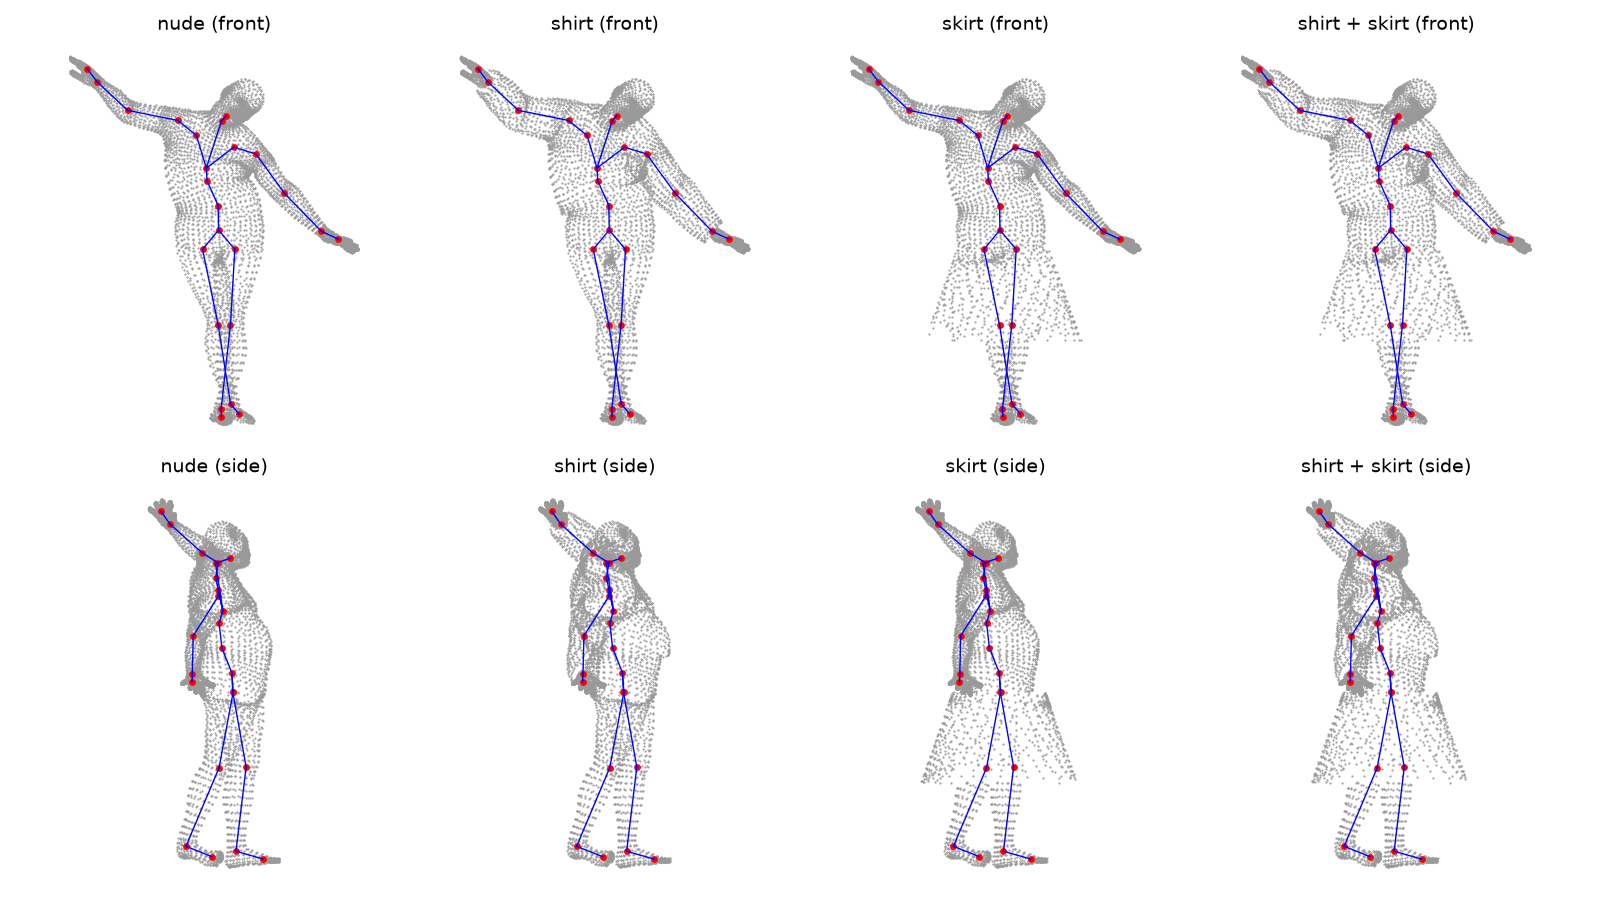
\includegraphics[width=\linewidth]{figures/synthetic_targets.png}
  \caption{Synthetic targets with their ground-truth skeleton: the same SMPL
  body nude, with a loose shirt, with a skirt, and with both (front and side
  views).}
  \label{fig:synthetic}
\end{figure}

\paragraph{Connectivity.} Without the check of Sec.~\ref{sec:connectivity} the
skirt splits the neighbourhood graph into two components (legs and body), and
the transfer collapses: on the first body the mean joint error is 832\,mm.
With the adaptive neighbourhood the same transfer has an error of 70\,mm.

% ----------------------------------------------------------------------------
\subsection{Skeleton priors and failure detection}
\label{sec:exp_failures}
% ----------------------------------------------------------------------------

Table~\ref{tab:priors} reports the error of the spectral transfer in the four
conditions. Loose clothing increases the error, and the combination of shirt
and skirt makes the transfer fail on most bodies.

\begin{table}[t]
  \centering
  \caption{Mean joint error (mm) of the spectral transfer on the synthetic
  benchmark (8 bodies per condition). The last two rows only include the
  transfers that pass the plausibility check.}
  \label{tab:priors}
  \begin{tabular}{lcccc}
    \toprule
    & nude & shirt & skirt & shirt + skirt \\
    \midrule
    All transfers                          & 27.5 & 42.0 & 94.9 & 337.8 \\
    Flagged as implausible                 & 0/8  & 2/8  & 5/8  & 7/8   \\
    \midrule
    Plausible transfers                    & 27.5 & 33.8 & 59.5 & 76.5  \\
    Plausible transfers + priors (Eq.~\ref{eq:priors}) & 26.0 & 32.4 & 57.6 & 75.4 \\
    \bottomrule
  \end{tabular}
\end{table}

\paragraph{Failure detection.} The plausibility check flags all the eight
transfers with an error above 10\,cm (up to 663\,mm), without using the ground
truth. It also flags six transfers with errors between 39 and 87\,mm, and the
largest error among the non-flagged transfers is 81\,mm. Inspecting the
failures shows that they are not left/right swaps (exchanging the labels of the
mirrored joints always increases the error) but partial collapses of the map,
where whole joints are transferred onto the wrong limb and some bones become
up to ten times longer than their true length.

\paragraph{Skeleton priors.} The priors consistently reduce the error of the
plausible transfers by about 5\% (Tab.~\ref{tab:priors}). The gain saturates for
$\omega_{sym}, \omega_{prop} \geq 1$: stronger weights do not help, and the
symmetry term alone does not help with clothing. The residual error is
therefore not explained by inconsistent bone lengths but by the placement of
the joints, and the large errors are failures of the correspondence that no
prior on the skeleton can repair. This motivates improving the correspondence
itself.

% ----------------------------------------------------------------------------
\subsection{Robust correspondence}
\label{sec:exp_robust}
% ----------------------------------------------------------------------------
% code: commit 20fc426, tools/benchmark_synthetic.py -n 6

We compare the components of Sec.~\ref{sec:robust} on six bodies per condition
(Tab.~\ref{tab:variants}). Every variant shares the target bases; the
combined variants also force the landmarks to correspond in every
point-to-point step, which alone has no measurable effect.

\begin{table}[t]
  \centering
  \caption{Mean (median) joint error in mm of the spectral transfer on the
  synthetic benchmark, 6 bodies per condition; failures are transfers with an
  error above 10\,cm; time per transfer, target basis excluded.}
  \label{tab:variants}
  \small
  \begin{tabular}{lccccrr}
    \toprule
    & nude & shirt & skirt & shirt + skirt & failures & time \\
    \midrule
    Baseline                 & 23.0 (22.8) & 55.0 (34.8) & 118.8 (81.0) & 227.9 (182.7) & 8/24 & 14\,s \\
    + limb landmarks         & 23.6 (22.8) & 55.8 (45.2) & 116.9 (73.0) & 190.1 (182.0) & 7/24 & 15\,s \\
    + restarts               & 23.0 (22.8) & 55.0 (34.8) &  99.6 (71.0) & 182.2 (110.1) & 6/24 & 34\,s \\
    + guided refinement      & 21.4 (20.2) & 55.7 (32.8) &  95.5 (64.6) & 229.9 (188.6) & 8/24 & 62\,s \\
    All three                & 22.0 (19.3) & 60.1 (42.8) &  51.2 (51.9) &  70.4 (68.2)  & 2/24 & 177\,s \\
    All three + priors       & \textbf{19.5} (17.1) & \textbf{54.8} (39.6) & \textbf{47.5} (50.6) & 71.0 (72.4) & 2/24 & 81\,s \\
    \bottomrule
  \end{tabular}
\end{table}

Each component alone gives a limited gain, but their combination is much
stronger than the sum of the parts: the skirt error drops from 118.8 to
47.5\,mm ($-60\%$), the shirt-and-skirt error from 227.9 to 71.0\,mm
($-69\%$), and the failures from eight to two. The refinement needs a
reasonable starting skeleton: alone it cannot recover from a collapsed map,
while after the restarts and with the limb landmarks it removes most of the
residual error, and the skeleton priors stabilize it (the iterations stop
earlier, hence the shorter time). The gain concentrates on the joints hidden
by the garments: for the skirt the leg error goes from 206.7 to 87.2\,mm and
the spine error from 99.9 to 37.4\,mm. The loose shirt is the exception: the
mean error does not change and the median increases, the legs being placed
worse (from 45.4 to 64.1\,mm) while the arms improve (from 61.6 to 48.0\,mm).
The knees remain the least accurate joints (120--141\,mm) when a garment
covers them.

\paragraph{Unsupervised diagnostics.} Table~\ref{tab:diagnostics} reports how
well each diagnostic of Sec.~\ref{sec:robust} predicts the true error over all
the intermediate results of all runs (771 stages). All of them are strongly
correlated with the error; the segment consistency has the highest rank
correlation, and the bone ratios, the symmetry and the segment consistency
separate the failures from the successful transfers with an area under the
ROC curve of 0.95--0.96.

\begin{table}[t]
  \centering
  \caption{Rank correlation (Spearman) of the unsupervised diagnostics with the
  true joint error, and area under the ROC curve for detecting failures
  (error $>$ 10\,cm), over 771 intermediate results.}
  \label{tab:diagnostics}
  \small
  \begin{tabular}{lcc}
    \toprule
    Diagnostic & Spearman $\rho$ & AUC (failures) \\
    \midrule
    Bone-ratio deviation             & 0.86 & 0.95 \\
    Mirrored-bone difference          & 0.79 & 0.96 \\
    Spectral / pointwise gap          & 0.81 & 0.84 \\
    Deviation from orthogonality      & 0.88 & 0.85 \\
    Coverage of the target            & 0.87 & 0.93 \\
    Segment consistency               & \textbf{0.89} & 0.95 \\
    \bottomrule
  \end{tabular}
\end{table}

\paragraph{Convergence.} The refinement does not reach a fixed point: after
four iterations the largest joint displacement oscillates around 6\% of the
mean bone length instead of vanishing, while the error has already reached a
plateau (with the refinement alone, from 106.2\,mm before the first iteration
to 100.3\,mm after the fourth and 100.6\,mm after the eighth). A threshold on
the displacement of the joints is therefore not a usable stopping criterion.
Choosing, among the iterates, the one with the best diagnostic does not help
either: the iterations improve the result almost monotonically, and the last
iterate (48.8\,mm for the combined variant, before the priors) is better than
the one selected by any diagnostic (49.3\,mm at best, with the segment
consistency), the best possible choice being 46.5\,mm. The diagnostics are
instead effective as a stopping criterion: stopping when the segment
consistency has not improved by more than $0.002$ for two consecutive
iterations gives 49.4\,mm with 5.4 iterations on average instead of 7.7.

\paragraph{Limitations.} The garments are simple geometric models, not cloth
simulations; the conclusions must be confirmed on real scans of clothed
people with ground-truth skeletons, e.g.\ CAPE~\citep{ma2020cape}.

\bibliographystyle{plainnat}
\bibliography{refs}

\end{document}
